\documentclass[12pt, times news roman, a4paper] {article}
\usepackage{graphicx}
\usepackage{caption}
\renewcommand{\figurename} {penjelasan}
\begin{document}
\begin{center}
	\LARGE{tugas data base}\\
	\noindent{Muh Amri Irianto (1184100)}
	
\end{center}
\section{Aplication express}
aplikasi expres adalah website yang dibuat oracle untuk membuat aplikasi secara cepat (express) fitur ini lebih mudah digunakan karena banyak yang menyangkut aplikasi cepat berikut langkah-langkahnya

\begin{enumerate}
	\item workspace : steam
	\item email     : amrijieces12@gmail.com
	\item password  : keren112
	
\end{enumerate}

\begin{minipage}{\linewidth}
	\centering
	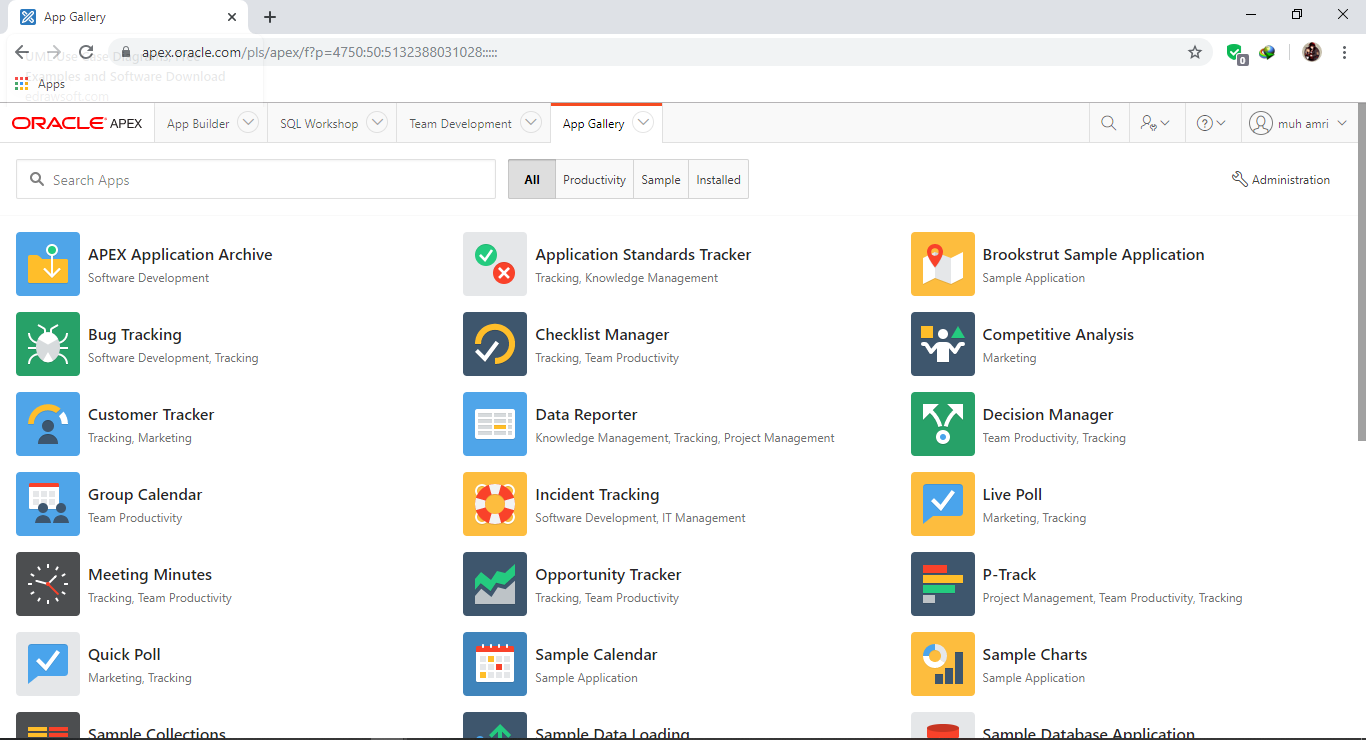
\includegraphics[width=12cm]{Gambar.png} 
	\captionof{figure} {pertama kita buat dulu file exclenya }
\end{minipage}

\begin{minipage}{\linewidth}
	\centering
	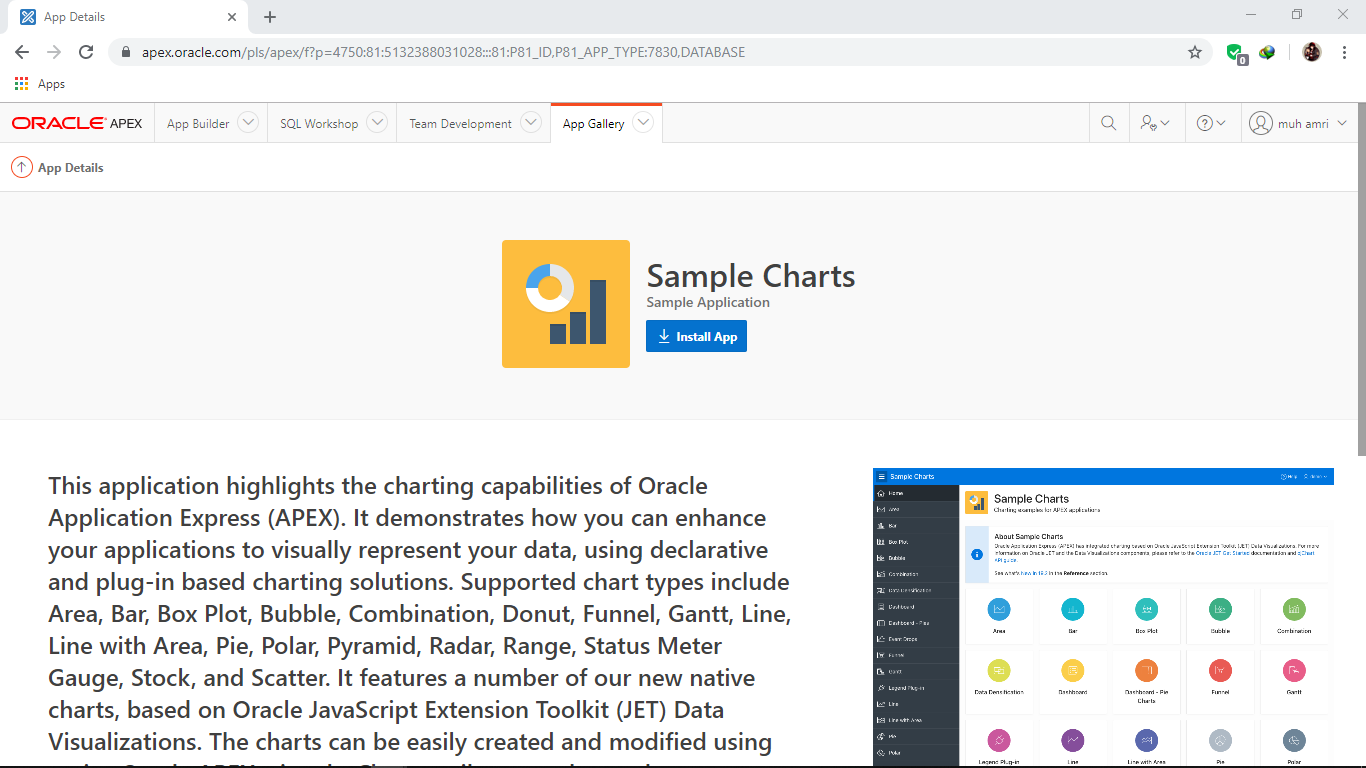
\includegraphics[width=12cm]{Gambar2.png} 
	\captionof{figure} {kita masuk keakun oracle yang sudah kita buat }
\end{minipage}

\begin{minipage}{\linewidth}
	\centering
	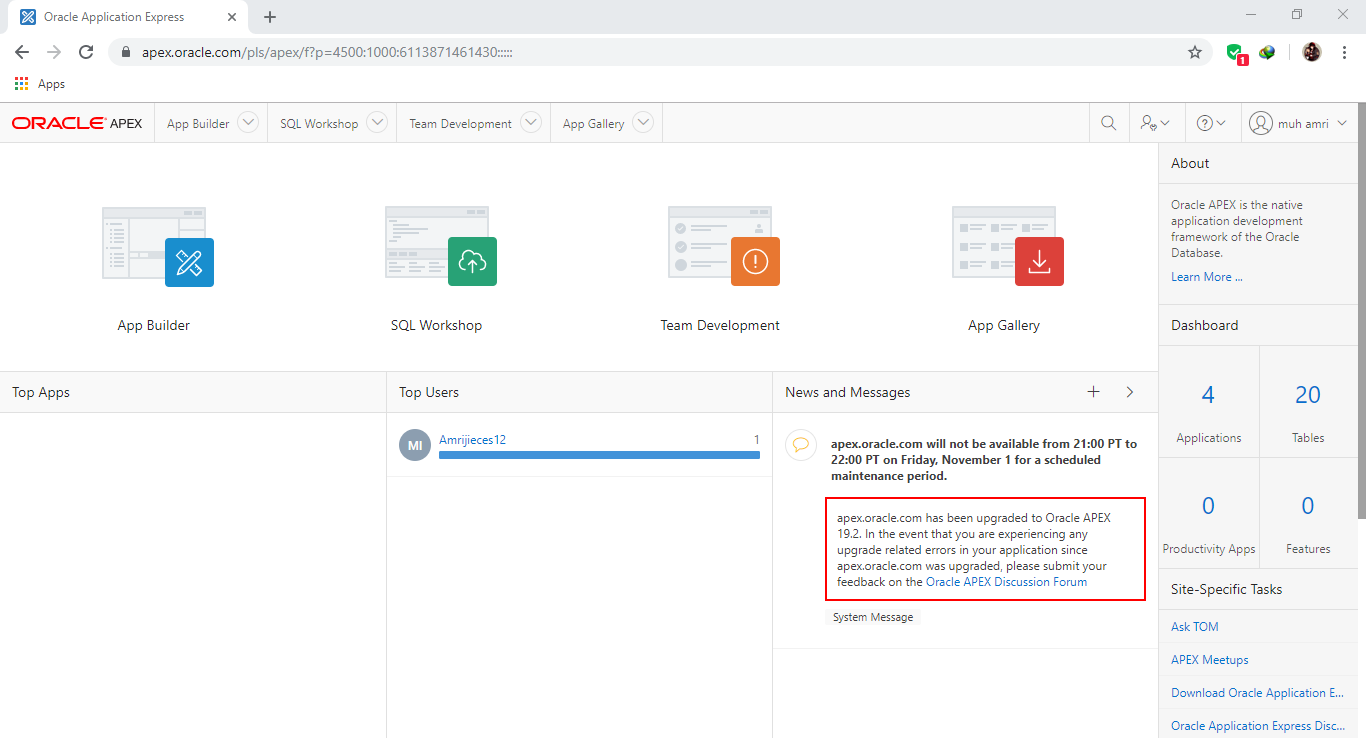
\includegraphics[width=12cm]{Gambar3.png} 
	\captionof{figure} {setelah kita masuk kita klick app builder }
\end{minipage}

\begin{minipage}{\linewidth}
	\centering
	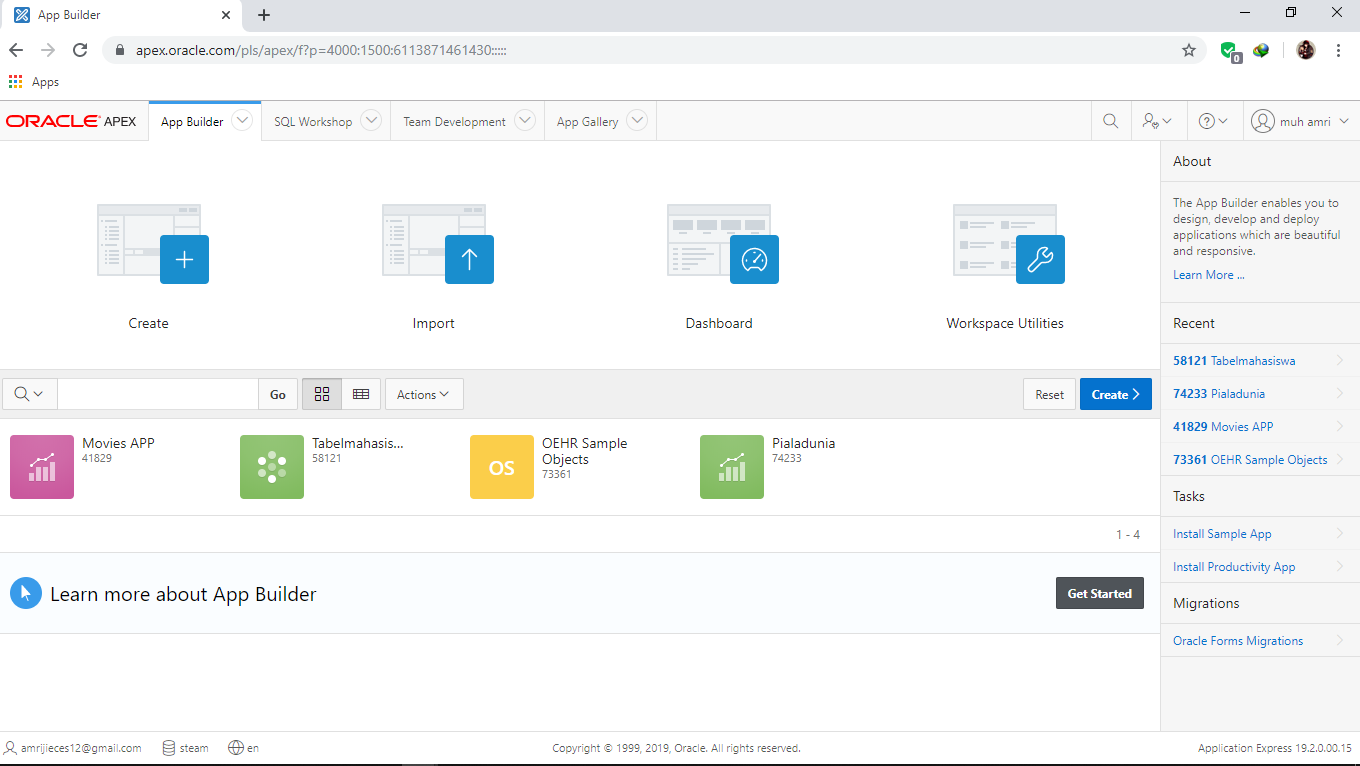
\includegraphics[width=12cm]{Gambar4.png} 
	\captionof{figure} {setelah kita masuk lalu klick create }
\end{minipage}

\begin{minipage}{\linewidth}
	\centering
	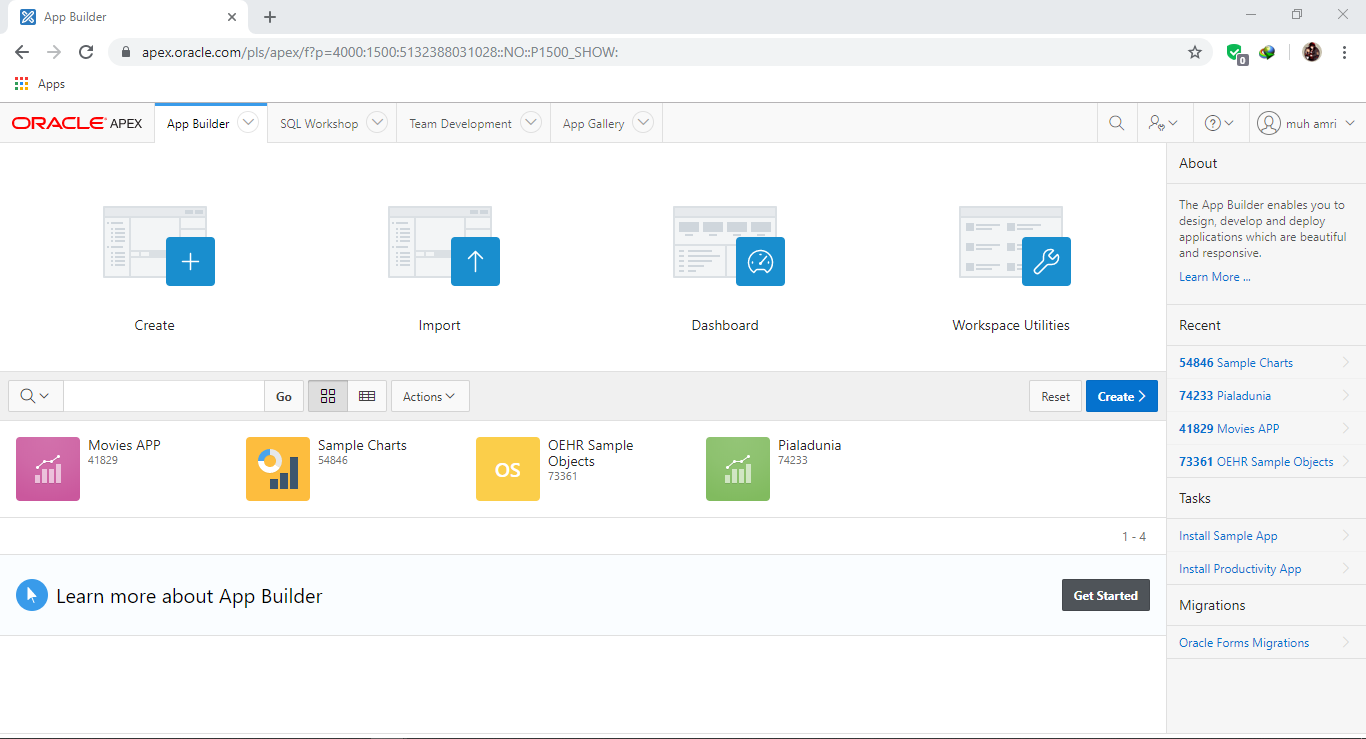
\includegraphics[width=12cm]{Gambar5.png} 
	\captionof{figure} {terus kita pilih from a file }
\end{minipage}

\begin{minipage}{\linewidth}
	\centering
	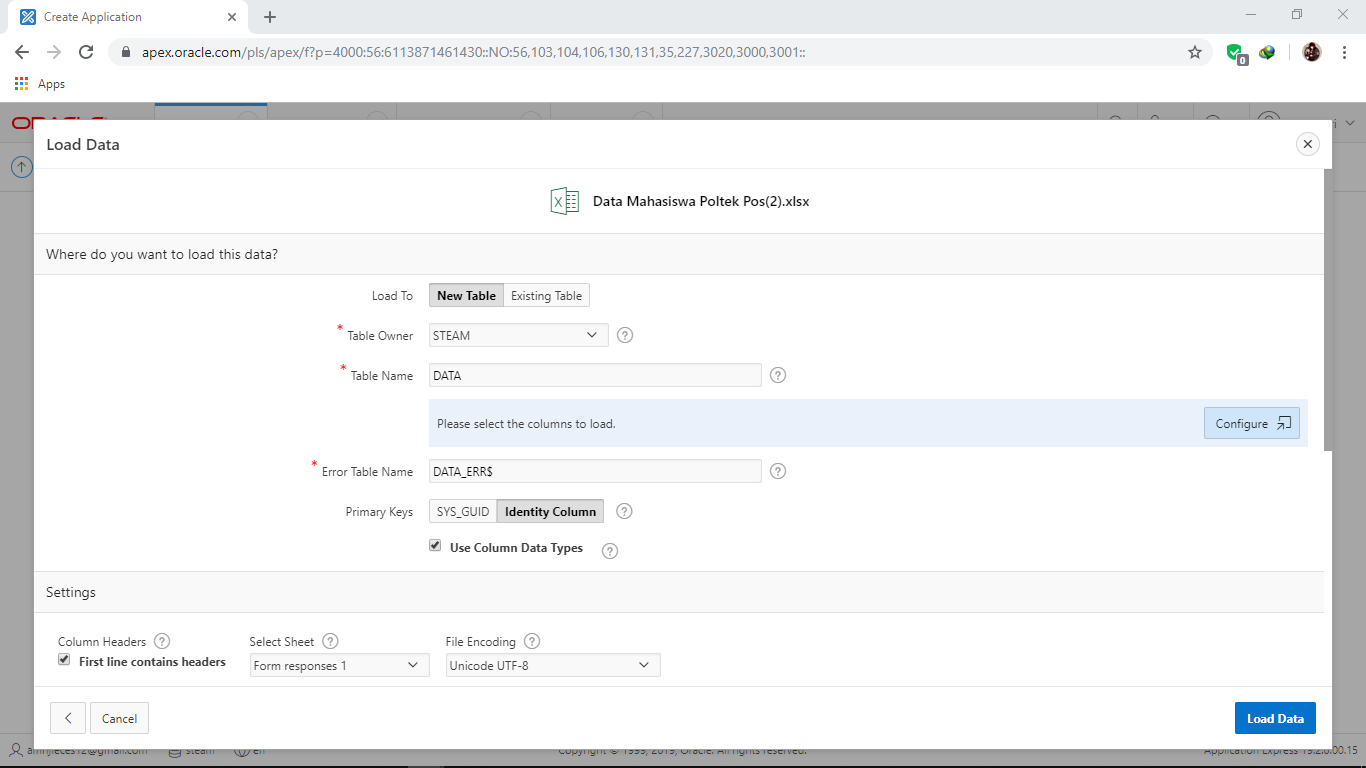
\includegraphics[width=12cm]{Gambar6.png} 
	\captionof{figure} {stelah kita masukkan chosenfile kita bisa masukkan nama aplikasi yang akan kita buat saya menggunakan nama "data" dan kita load data }
\end{minipage}

\begin{minipage}{\linewidth}
	\centering
	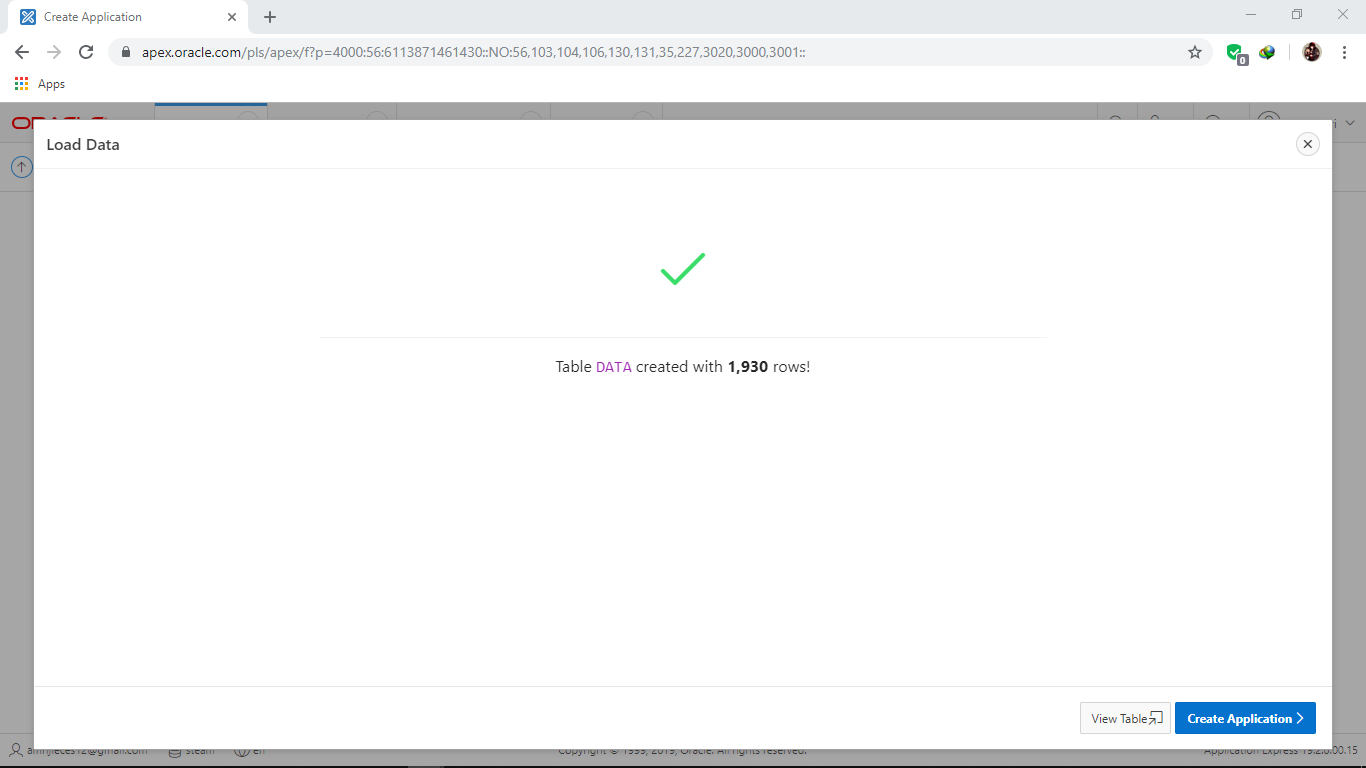
\includegraphics[width=12cm]{Gambar7.png} 
	\captionof{figure} {terus kita tunngu tunggu kita klick create application}
\end{minipage}

\begin{minipage}{\linewidth}
	\centering
	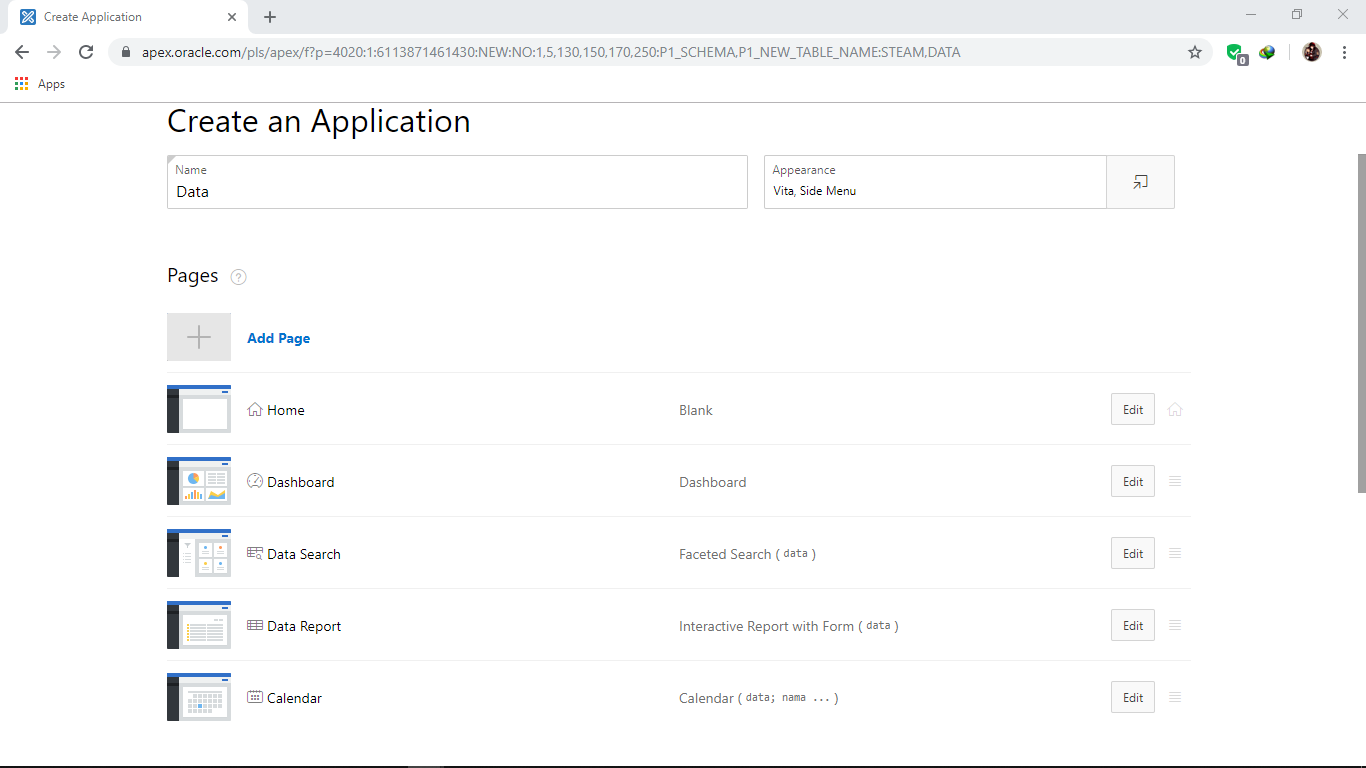
\includegraphics[width=12cm]{Gambar8.png} 
	\captionof{figure} {kita scrool ke paling bawah terus kita pilih create application }
\end{minipage}

\begin{minipage}{\linewidth}
	\centering
	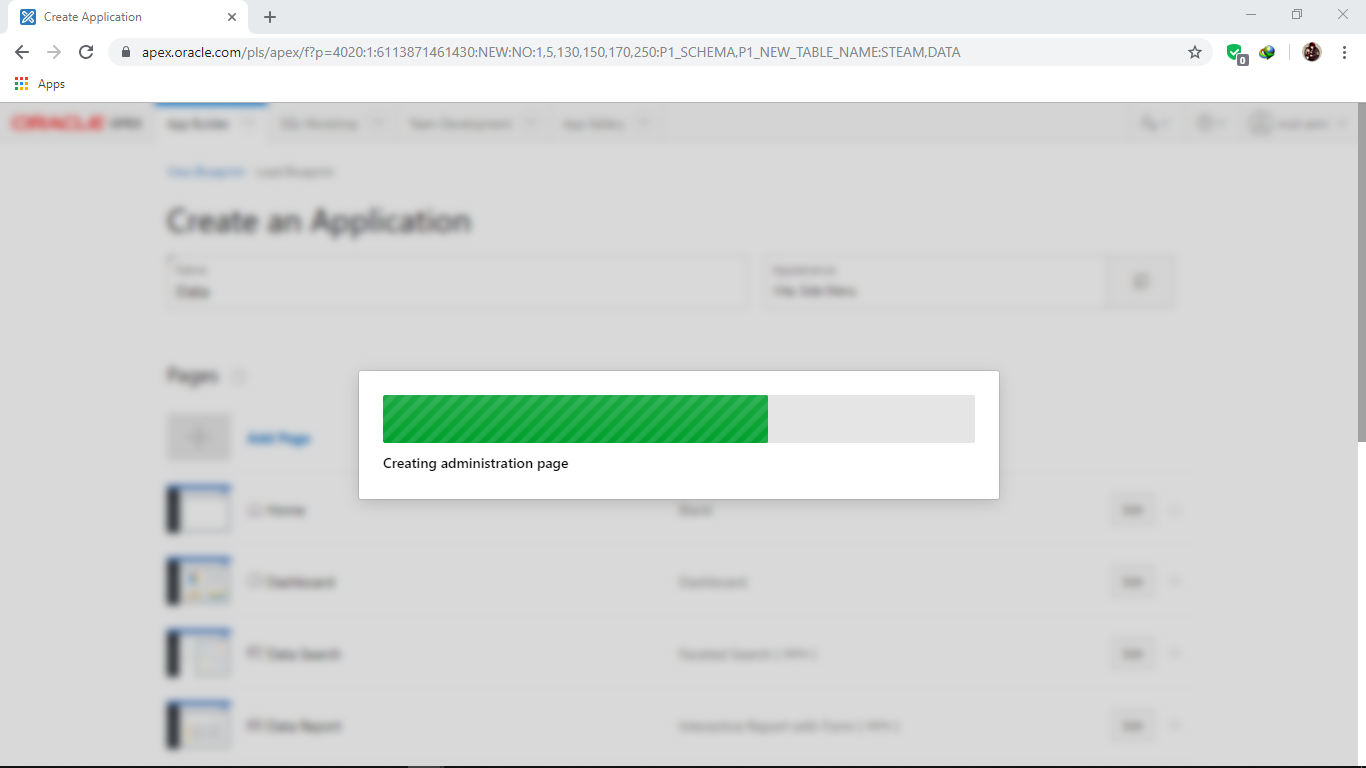
\includegraphics[width=12cm]{Gambar9.png} 
	\captionof{figure} {kita tunngu}
\end{minipage}

\begin{minipage}{\linewidth}
	\centering
	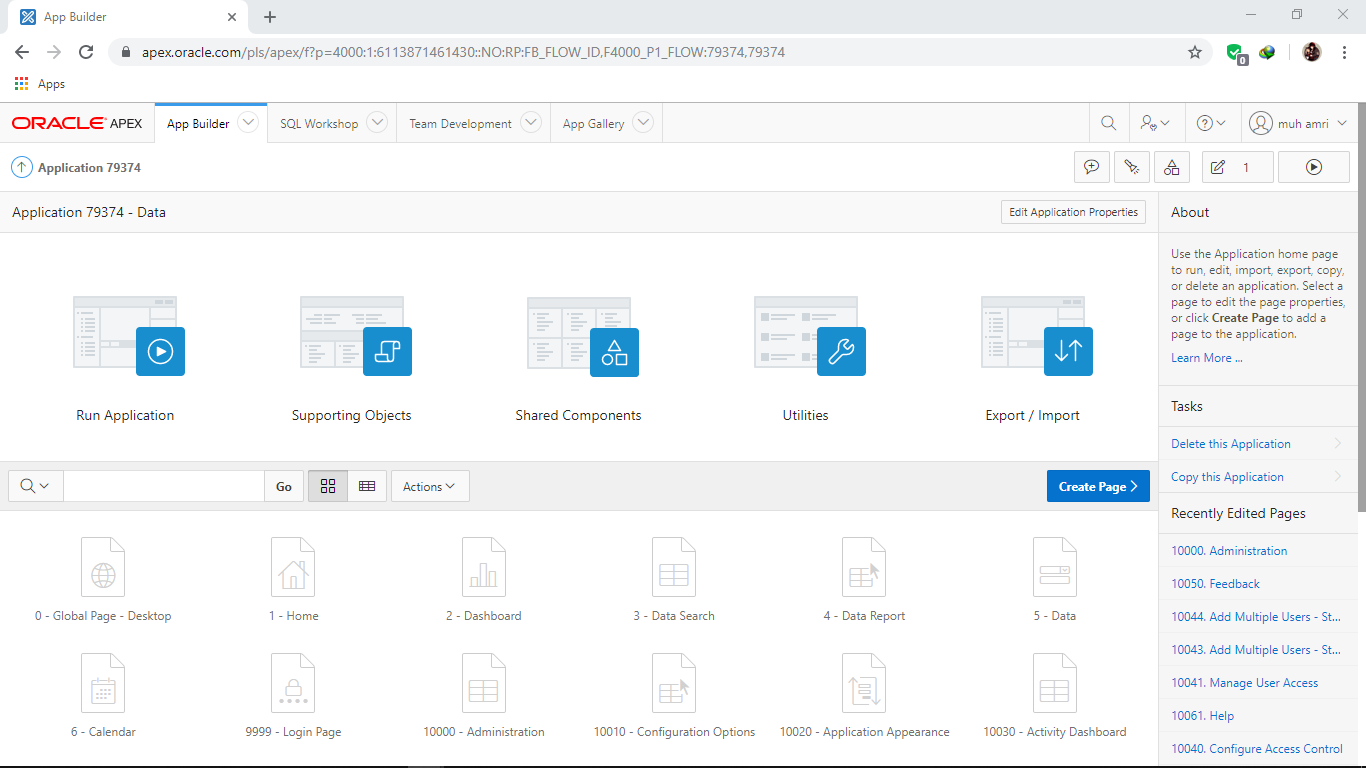
\includegraphics[width=12cm]{Gambar10.png} 
	\captionof{figure} {kita akang otomatis diarah daiarahkan ke app builer dan kita click run application }
\end{minipage}

\begin{minipage}{\linewidth}
	\centering
	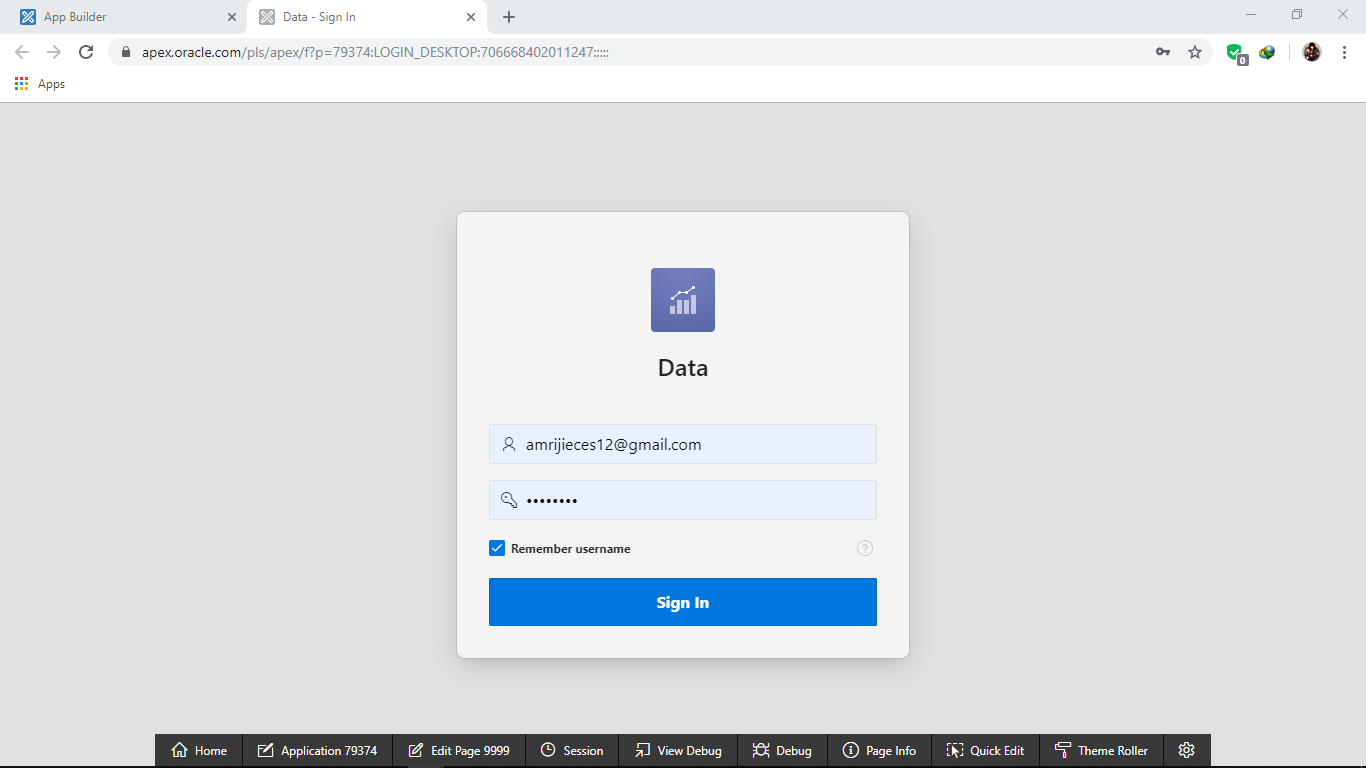
\includegraphics[width=12cm]{Gambar11.png} 
	\captionof{figure} {terus kita sigin in untuk app kita }
\end{minipage}

\begin{minipage}{\linewidth}
	\centering
	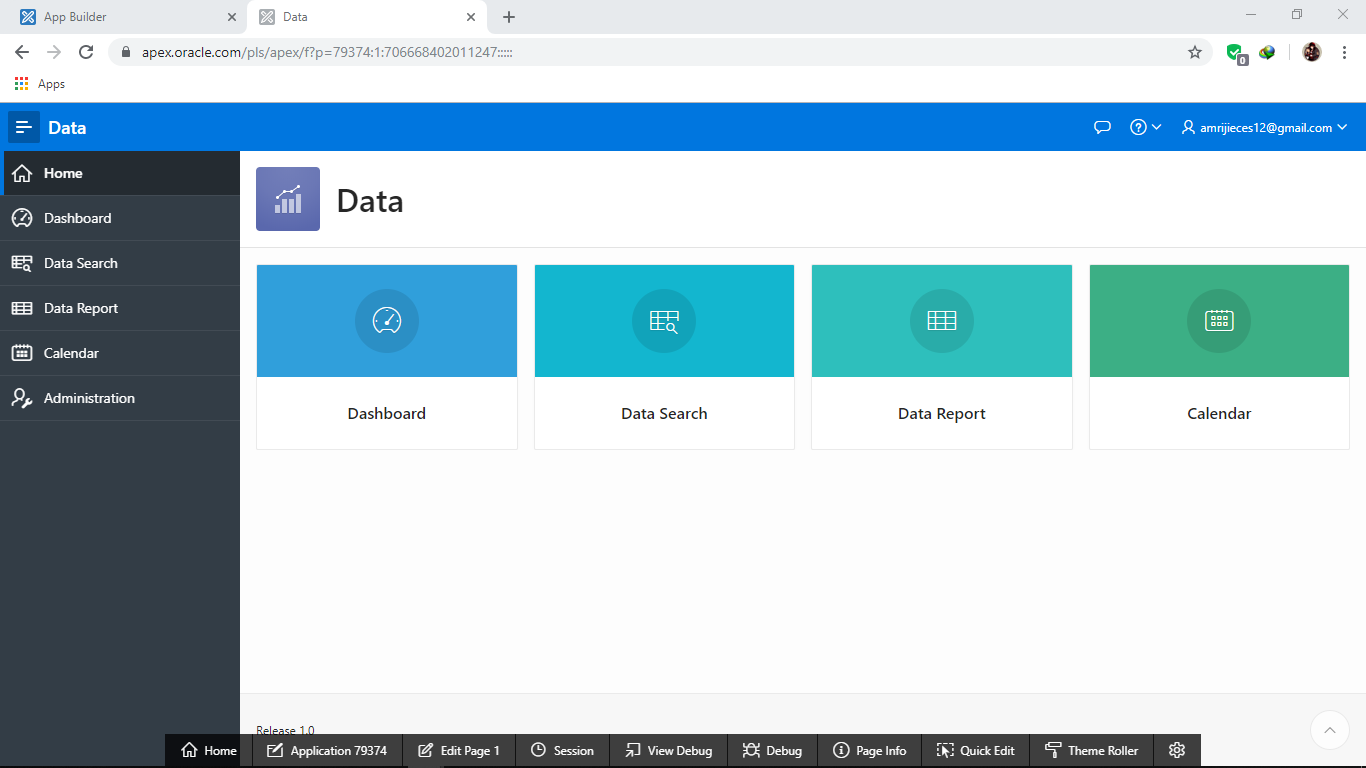
\includegraphics[width=12cm]{Gambar12.png} 
	\captionof{figure} {dan selesai kita lakukan } 
\end{minipage}

\end{document}